\NeedsTeXFormat{LaTeX2e}[1995/12/01]
\documentclass[10pt]{bmc_article}    



% Load packages
\usepackage{cite} % Make references as [1-4], not [1,2,3,4]
\usepackage{url}  % Formatting web addresses  
\usepackage{ifthen}  % Conditional 
\usepackage{multicol}   %Columns
\usepackage[utf8]{inputenc} %unicode support
%\usepackage[applemac]{inputenc} %applemac support if unicode package fails
%\usepackage[latin1]{inputenc} %UNIX support if unicode package fails
\urlstyle{rm}
 
%%%%%%%%%%%%%%%%%%%%
%% Karro macros   %%
%%%%%%%%%%%%%%%%%%%%
\newcommand{\peace} {{\small PEACE}}
\newcommand{\wcd} {{\small WCD}}
\newcommand{\capthree} {{\small Cap3}}
\newcommand{\easycluster} {{\small EasyCluster}}
\newcommand{\estsim}{{\small ESTSim}}
\newcommand{\metasim} {{\small MetaSim}}
\newcommand{\tgicl} {{\small TGICL}}
\newcommand{\east} {{\small EAST}}
\newcommand{\velvet}{{\small Velvet}}
\newcommand{\mira}{{\small Mira3}}
\newcommand{\pave} {{\small PAVE}}
\newcommand{\peast}{{\small PEACE+EAST}}
 
%%%%%%%%%%%%%%%%%%%%%%%%%%%%%%%%%%%%%%%%%%%%%%%%%	
%%                                             %%
%%  If you wish to display your graphics for   %%
%%  your own use using includegraphic or       %%
%%  includegraphics, then comment out the      %%
%%  following two lines of code.               %%   
%%  NB: These line *must* be included when     %%
%%  submitting to BMC.                         %% 
%%  All figure files must be submitted as      %%
%%  separate graphics through the BMC          %%
%%  submission process, not included in the    %% 
%%  submitted article.                         %% 
%%                                             %%
%%%%%%%%%%%%%%%%%%%%%%%%%%%%%%%%%%%%%%%%%%%%%%%%%                     

\usepackage{graphicx}
%\def\includegraphic{}
%\def\includegraphics{}


\setlength{\topmargin}{0.0cm}
\setlength{\textheight}{21.5cm}
\setlength{\oddsidemargin}{0cm} 
\setlength{\textwidth}{16.5cm}
\setlength{\columnsep}{0.6cm}

\newboolean{publ}

%%%%%%%%%%%%%%%%%%%%%%%%%%%%%%%%%%%%%%%%%%%%%%%%%%
%%                                              %%
%% You may change the following style settings  %%
%% Should you wish to format your article       %%
%% in a publication style for printing out and  %%
%% sharing with colleagues, but ensure that     %%
%% before submitting to BMC that the style is   %%
%% returned to the Review style setting.        %%
%%                                              %%
%%%%%%%%%%%%%%%%%%%%%%%%%%%%%%%%%%%%%%%%%%%%%%%%%%
 

%Review style settings
\newenvironment{bmcformat}{\begin{raggedright}\baselineskip20pt\sloppy\setboolean{publ}{false}}{\end{raggedright}\baselineskip20pt\sloppy}

%Publication style settings
%\newenvironment{bmcformat}{\fussy\setboolean{publ}{true}}{\fussy}



% Begin ...
\begin{document}
\begin{bmcformat}

\title{EAST: {\underline E}xpression Fragment {\underline A}ssembly from {\underline S}panning {\underline T}rees}

%%%%%%%%%%%%%%%%%%%%%%%%%%%%%%%%%%%%%%%%%%%%%%
%%                                          %%
%% Enter the authors here                   %%
%%                                          %%
%% Ensure \and is entered between all but   %%
%% the last two authors. This will be       %%
%% replaced by a comma in the final article %%
%%                                          %%
%% Ensure there are no trailing spaces at   %% 
%% the ends of the lines                    %%     	
%%                                          %%
%%%%%%%%%%%%%%%%%%%%%%%%%%%%%%%%%%%%%%%%%%%%%%


\author{Yuan Zhang$^1$
  \email{Yuan Zhang - zhangy9@muohio.edu}
  \and
  James C Moler$^1$
  \email{James Moler - molerjc@muohio.edu}
  \and
  Dhananjai M Rao$^1$
  \email{Dhananjai Rao - raodm@muohio.edu}
  \and
  Mufit Ozden$^1$
  \email{Mufit Ozden - ozdenm@muohio.edu}
  \and
  Chun Liang\correspondingauthor$^{1,2}$
  \email{Chun Liang\correspondingauthor - liangc@muohio.edu}
  and
  John E. Karro\correspondingauthor$^{1,3}$
  \email{John E. Karro\correspondingauthor - karroje@muohio.edu}
}

%%%%%%%%%%%%%%%%%%%%%%%%%%%%%%%%%%%%%%%%%%%%%%
%%                                          %%
%% Enter the authors' addresses here        %%
%%                                          %%
%%%%%%%%%%%%%%%%%%%%%%%%%%%%%%%%%%%%%%%%%%%%%%

\address{
    \iid(1)Department of Computer Science and Software Engineering, Miami University, Oxford OHIO, USA \\
    \iid(2)Department of Botanty, Miami University, Oxford OHIO, USA \\
    \iid(3)Department of Microbiology, Miami University, Oxford OHIO, USA
}

\maketitle

%%%%%%%%%%%%%%%%%%%%%%%%%%%%%%%%%%%%%%%%%%%%%%
%%                                          %%
%% The Abstract begins here                 %%
%%                                          %%
%% The Section headings here are those for  %%
%% a Research article submitted to a        %%
%% BMC-Series journal.                      %%  
%%                                          %%
%% If your article is not of this type,     %%
%% then refer to the Instructions for       %%
%% authors on http://www.biomedcentral.com  %%
%% and change the section headings          %%
%% accordingly.                             %%   
%%                                          %%
%%%%%%%%%%%%%%%%%%%%%%%%%%%%%%%%%%%%%%%%%%%%%%


\begin{abstract}
        % Do not use inserted blank lines (ie \\) until main body of text.
\end{abstract}



\ifthenelse{\boolean{publ}}{\begin{multicols}{2}}{}




%%%%%%%%%%%%%%%%%%%%%%%%%%%%%%%%%%%%%%%%%%%%%%
%%                                          %%
%% The Main Body begins here                %%
%%                                          %%
%% The Section headings here are those for  %%
%% a Research article submitted to a        %%
%% BMC-Series journal.                      %%  
%%                                          %%
%% If your article is not of this type,     %%
%% then refer to the instructions for       %%
%% authors on:                              %%
%% http://www.biomedcentral.com/info/authors%%
%% and change the section headings          %%
%% accordingly.                             %% 
%%                                          %%
%% See the Results and Discussion section   %%
%% for details on how to create sub-sections%%
%%                                          %%
%% use \cite{...} to cite references        %%
%%  \cite{koon} and                         %%
%%  \cite{oreg,khar,zvai,xjon,schn,pond}    %%
%%  \nocite{smith,marg,hunn,advi,koha,mouse}%%
%%                                          %%
%%%%%%%%%%%%%%%%%%%%%%%%%%%%%%%%%%%%%%%%%%%%%%




%%%%%%%%%%%%%%%%
%% Background %%
%%
\section*{Introduction}
The {\it de novo} assembly of RNA transcripts is an important and
computationally challanging problem, made more difficult by the advent
of Next Generation Sequencing technologies such as 454 or Illumina
[CITE].  Given the completion of large-scale seqencing run of multiple
mature transcripts of a given organism, the invetigator is left with a
large set of sequence fragments, but no ordering or even transcript
association information; these fragments must be clustered by
transcript then assembled before the sequencing output can be truely
useful.  If the genome has not been sequenced, this must be done {\it
  de novo} -- using only the sequence information extrapolated from
the sequences themselves.  Even when the genomic sequence is known,
there are a number of advanatages to ignoring the known sequence
information and starting from scratch.  Using an existing squence as a
template for sequencing in population studies has the potential to
introduce bias.  And when looking specifically for genes, a known
sequence may be of limited use: the target transcripts may be
undiscovered, and the splicing of introns before sequencing can complicate
the approach of mapping fragemtns to the genomic sequence.  In short,
there is significant value in tools that can reassemble fragement data
into the orginial assembly without requiring access to genomic
information.

The problem of {\it de novo} transcript assembly has been addressed a number
of times in the literature, with initial approaches consentrating on
the longer reads produced by traditional Sanger Sequencing techniques,
and newer approaches looking at produces of Next Generation Sequencing
(NGS) technologies.  A list of the tools most successfully addressing
these problems include \capthree, \tgicl, \velvet, and \mira [CITE],
each excelling within their own context.  \capthree\/ and \tgicl\/ use
alignment-based strategies that produce high quality results when
applied to the output of Sanger sequencing technologies.  \velvet,
based on the modeling of the problem with a {\it de bruijn} graphs,
was designed to handle short read sequences.  [SOMETHING ABOUT MIRA --
INCLUDING ABIITY TO HANDLE HYBRID DATA.]


In this paper we present \east, a tool for the assembly of both
Sanger, NGS and hybrid data with the capacity to incorperate quality
scores when available.  \east\/ is based on a novel minimum spanning
tree (MST) apraoch to compute assembly.  The tool works in tandem with
the \peace\/ clustering tool [CITE] -- allowing \peace\/ to cluster
fragements by transcript and produce the initial MSTs that will serve
as the basis for the \east\/ algorithm.  In the following we present a
comparison of \east\/ against those of \capthree, \tgicl, \velvet, and
\mira on both Sanger and NGS sequences, showing that [???]



 
%%%%%%%%%%%%%%%%%%%%%%%%%%%%
%% Results and Discussion %%
%%
\section*{Results and Discussion}

In assessing result quality, we must view the \peace\/ clustering tool
\cite{Rao10} and \east\/ as a combined process.  While most assembly
tools integrate these two jobs, \east\/ assumes clustering has been
preformed and requires the \peace\/ MST output.  Hence for purposes of
the following section, we consider a single tool \peast, and
assess the quality of these results.

In order to assess the quality of the \east\/ (\peast\/) results, we compared
against four prominent assembly tools: \capthree, \tgicl,
\mira, and \velvet [CITE].  Tools were tested on data from three
sequencing technologies (Sanger, 454 and Illumina), using both
simulated output obtained from the \estsim\/ and \metasim\/ tools
[CITE] and benchmark sets obtained from GenBank [CITE].  


\subsection*{Measuring Quality}
Our primary measure of quality was the {\bf normalized A-score}, based
on the {\it assembly score} (A-score) used in {\it Liang et al.}
\cite{Liang00}.  For an assembly of some originial sequence, the
A-score is defined as:
$$\mbox{($2\times$sequence length) - ($5\times$ number of
mismatches) - ($15 \times$ number of indels)}$$
with a ``perfect'' score equal to twice the sequence length.  Our
normalized A-score modifies this definition as:
$$\frac{\mbox{($2\times$assembly length) - ($5\times$ number of mismatches)
  - ($15\times$ number of indels)}}{\mbox{($2\times$ sequence length)}}$$
with a perfect score equal to 1.  This normalization allows for the
comparison of assembly quality between sequences of differenct
lengths. Further, using this score we can more accurately quantify the
quality of a partial reconstrction: if we are able to reconstruct only
a portion of a fragment, the normalized A-score will take full
consideration of the quality of the reconstruction, but then bound the
score by the relative size of the reconstruction.  (e.g. Perfectly
reconstructiong one fourth of the original sequence will lead to an a
score of $0.25$.)  

In addition to A-score...

\subsection*{Simulation Results}
Using simulated fragement sets allows us to both compare assemblies to
a known correct solution and control parameters in their model
(e.g. base-call error rate) to test the effect of variation.  All sets
were generated from a set of 100 zebra fish transcripts obtained from
{\it Hazelhurst et al.}  \cite{Hazelhurst08}.  For simulated Sanger
sequences we used the \estsim\/ tool, using its default model of EST
generation and error rate when not otherwise specified.  For simulated
454 and Illumina sets we used the \metasim\/ tool, again using their
default model to simulate the errors associated with those
technologies.

\noindent {\bf Sanger Sequencing:} We start by looking at the assembly
quality of each tool, when applied to simulated Sanger Sequences, as a
function of error rate for a range of coverage depths.  For each
parameter combination we applied each tool to 30 independently
randomly generated simulated sets, derived from 15 zebra fish genes,
reporting the average normalized A-score.  In
Figure~\ref{sangerAscore} we look at normaized A-score as a function
of error rate, fixing coverage at 50, 30 and 10 and varying base-read
error rate from 0\% to 6\% [WHAT IS INDEL RATE?] for each of the five
tools being tested.  While the three illustrated tools preform well
when applied error free (i.e. impossible) sequencing technoloy, we
find \east\/ to be considerably more robust to base-call errors than the
other tools.  Taking the mid-range coverage value of 30 as an example,
at a 1\% error rate we see \east, \capthree, and \tgicl\/ all achieving an
essentially perfect normalize A-score, while \mira\/ ranges around a 0.5
and \velvet\/ does quite poorly.  At a 3\% error rate \east\/ maintains its
almost perfect normalized A-score, showing a 2\% improvement of \tgicl,
a 21\% improvlement over \capthree, and a 133\% improvement over \velvet.
At a 4\% error rate \east\/ still maintains its near-perfect score
(showing a 54\% and 85\% improvement over \capthree\/ and \tgicl\/
respecitvally), and even at a 6\% error rate is still achieving an
normalized A-score of 0.95 (a 110\% improvement over the next closest
tool, \tgicl\/).


\begin{figure}[htb]
\centerline{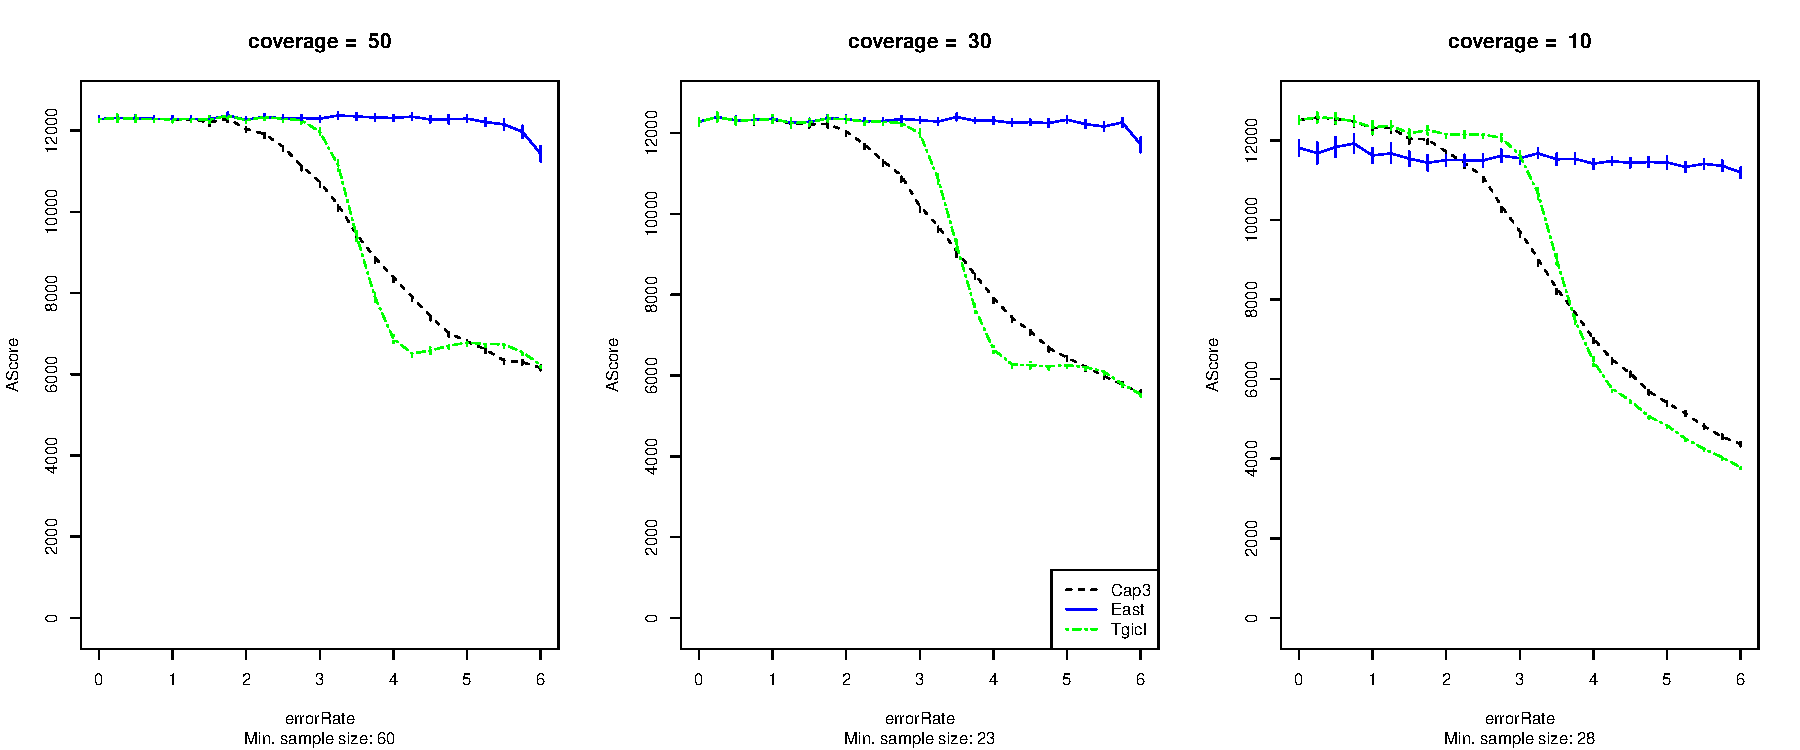
\includegraphics[width=6in]{pics.d/ascore_sanger.png}}
\label{sangerAscore}
\caption{Normalized a-score as a function of base error rate for
  simmulated sanger sequencing.  \east=blue, \capthree=Black,
  \tgicl=green, \velvet=red, \mira=purple.}
\end{figure}

Another useful metric is the number of contigs and number of singleton
fragments in the final result.  In Figure~\ref{contigs.sanger} is a
plot of the average number of contigs per gene seqence (left column), ad
the number of singletons (right column).  For the first we observe that all tools have
comperable results for lower error rates, but only \east\/ is able to
maintain the low score with increasing error rates.  In minimizing the
number of singletons, we find that \east\/ does a better job than
\capthree\/ for error rates larger than $2\%$, while TGICL does a
better job that \east\/ for error rates larger than $4\%$ to $5\%$.

\begin{figure}[htb]
\begin{minipage}{3in}
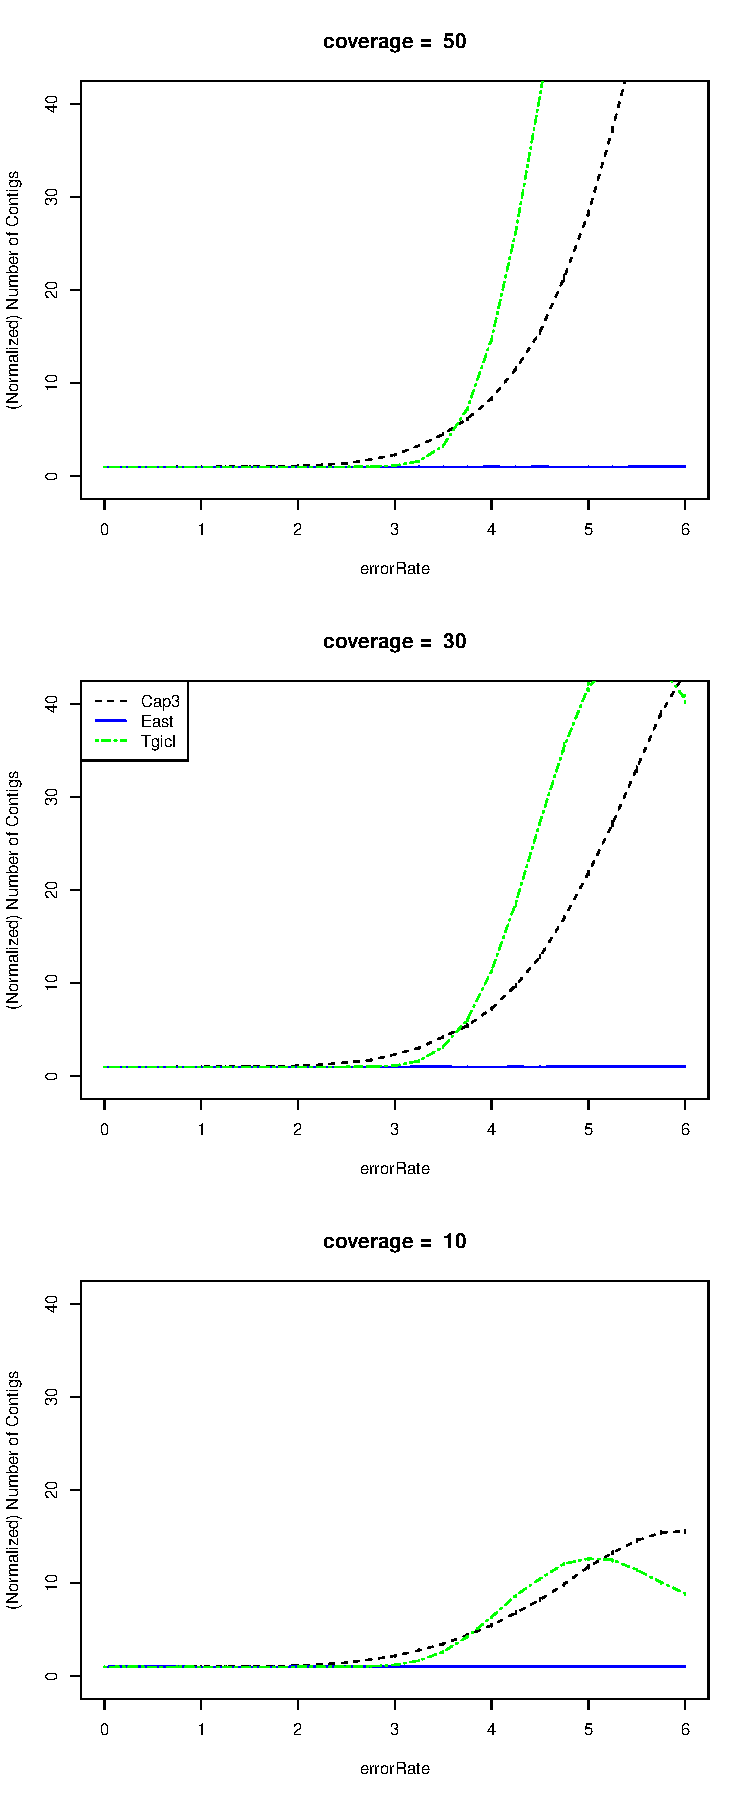
\includegraphics[width=3in]{pics.d/numContigs_sanger.png}
\end{minipage}
\begin{minipage}{3in}
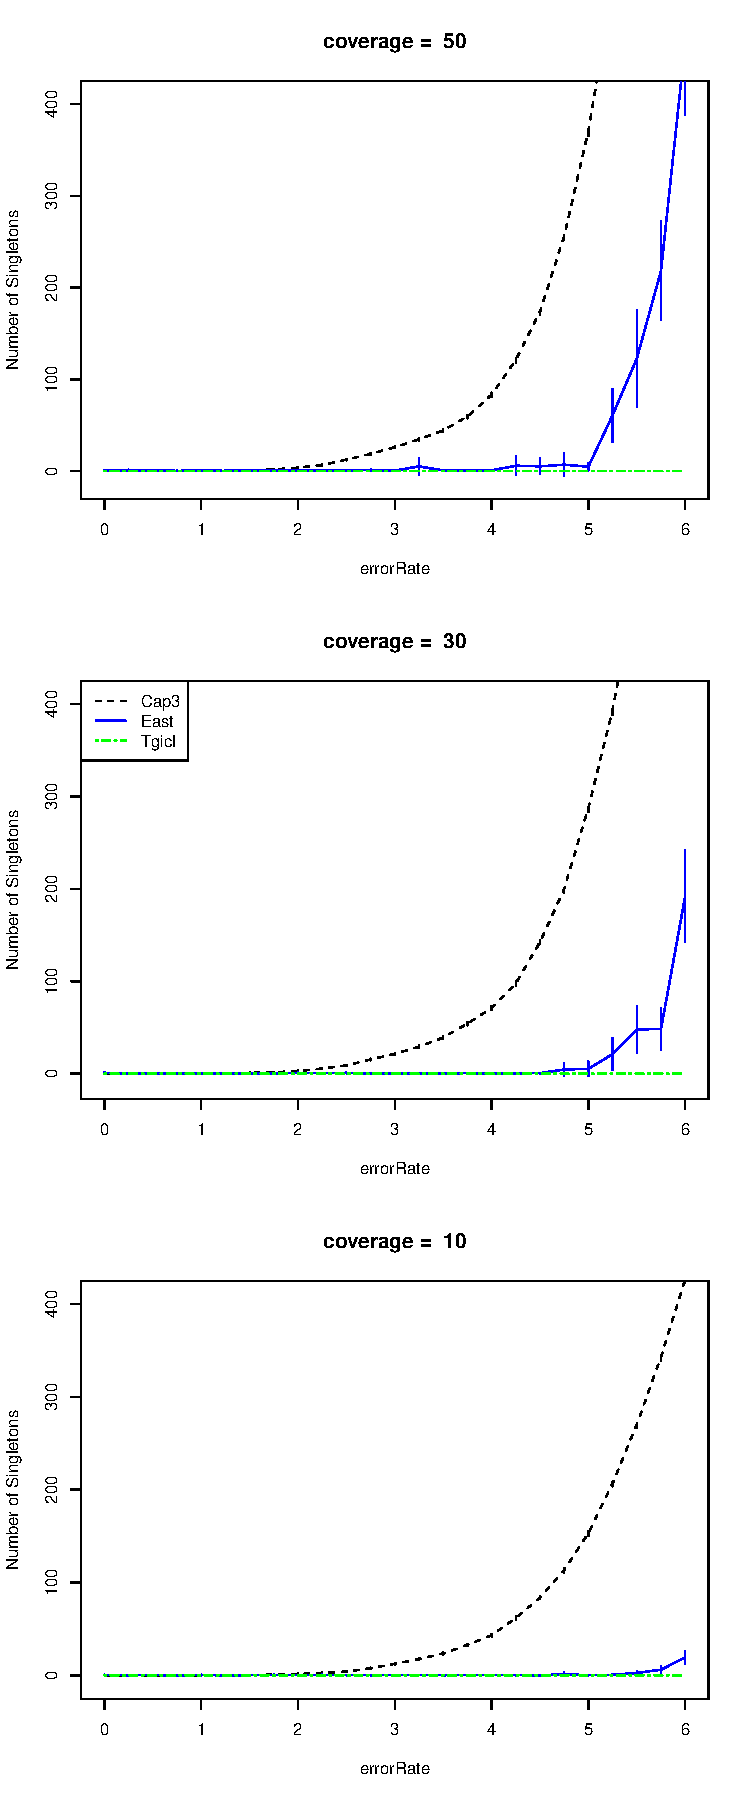
\includegraphics[width=3in]{pics.d/numSingle_sanger.png}
\end{minipage}
\label{contigs.sanger}
\caption{Number of contigs and singles as a function of base error
  rate for simmulated sanger sequencing.  \east=blue, \capthree=Black,
  \tgicl=green, \velvet=red, \mira=purple.  (Number of singles for
  \velvet\/ and \mira\/ not shown.)}
\end{figure}

[ADD SOMETHING ABOUT COVERAGE?  The situation is strange.]

\noindent {\bf Next Generation Sequences:} 








%%%%%%%%%%%%%%%%%%%%%%
\section*{Conclusions}


  
%%%%%%%%%%%%%%%%%%
\section*{Methods}

The algorithm underlying \east\/ is based on three components: minimum
spanning trees (MSTs)\cite{Prim57}, the $d^2$ sequence distance
measure \cite{Hide94}, and standard sequence alignment
\cite{Needleman70,Smith81}.  While we would ideally be using sequence
alignment to identify overlapping ends and reassembling on that basis,
the quadratic run time of alignment algorithms coupled with the large
number of sequences makes such an approach infeasible.  To avoid excessive
applications of such algorithms, we make use MSTs to provide a {\it
  guide} through the EST set, dictating which pairs we aligned.  A
modified version of the $d^2$ measure provides the edge weights for
the underlying graph, allowing us to define the MST and also providing
some speedup to the alignment algorithm.

\east\/ is technically an assembly tool, and require clustering be
done as a pre-processing step, as well as requiring that $d^2$-based
MSTs be provided for each cluster.  Conveniently, the \peace\/
clustering tool \cite{Rao10} provides exactly this information.  While
\peace\/ an \east\/ are technically two tools, \east\/ was designed
specifically for \peace\/ output.  For purposes of this paper, it
makes sense to consider them as one.  In the following we briefly
outline the \peace\/ algorithm for clustering (as is relevant to
\east\/), and then discuss the steps taken by \east\/ for assembly of
the \peace\/ clusters.

\subsection*{Clustering}

Given a set of fragments from two or more transcripts, we must first
cluster the fragments by transcript association -- leaving us with a
single cluster of fragments for each transcript.  Details of the
\peace\/ algorithm can be found in {\it Rao et al.} \cite{Rao10}, but
the general idea is as follows: we model the problem as a weighted,
undirected graph, representing each fragment with a node and assigning
edge weights based on a $d^2$ comparison of the incident fragments
(explained in more detail below).  By employing the $u/v$ and $t/v$
filtering heuristics of {\it Hazelhurst et al.} \cite{Hazelhurst08}, we
can quickly dismiss most of the edges as irrelevant (i.e. connecting
nodes that belong in different clusters), then use Prim's algorithm to
compute an MST \cite{Prim57}.  We then remove all
edges exceeding a specified threshold value, and take each component
of the resulting forest as a cluster.  As a result \peace\/ can pass
to \east\/ a set of clusters, an MST for each cluster, and the
orientation of each fragment relative to the cluster.  Hence \east\/
has not only the clusters, but the \peace\/ MST and may quickly adjust
the sequences to ensure all are on the same strand.

\subsection*{Overlap Detection}

Given the \peace\/ generated MST for a cluster, the challenge is to
identify and align the ends of overlapping fragments without taking
the significant run time hit needed to align every pair.  We
accomplish this using two methods: we reduce the number of times an
alignment is calculated aligning only those sequences adjacent in the
MST, and we reduce the amount of  time spent per alignment by aligning
only those portions indicated by an application of a modified form of
the $d^2$ sequence distance measure.

The presence of an edge in the tree is a heuristic indication that the
incident sequences overlap; were there not sufficient sequence
similarity to indicate an overlap, the edge would have been assigned a
high $d^2$ value and would have been removed by \peace\/.  To
determine how the nodes overlap, we calculate a modified $d^2$ score
as follows.  The standard calculation of $d^2$, as define by {\it Hide
  et al.} \cite{Hide94}, requires looking at every pair of length $w$
sub-strings (windows) from the two sequences, calculating a distance
between these two windows based on the number of shared words
(6-mers), and taking the score of the lowest-scoring window pairs as
the $d^2$ distance.  However, when looking for overlap of fragments
$s_1$ and $s_2$, we are looking only for end-overlap.  That is, we
wish to determine of the left end of $s_1$ overlaps the right end of
$s_2$, or the reverse (recalling that we know them to be on the same
strand).  Hence we need only consider the left-most and right-most
windows of $s_1$ against each window of $s_2$, reducing the number of
window comparisons from quadratic to linear in the size of $s_2$.

In Figure~\ref{fig:overlap} we see illustrate the use of modified $d^2$,
using it to take two sequences (a), find the window on $s_2$ most
resembling the right-most window of $s1$ (red section of (b)),
extending to the end of $s_2$ (green section of (c)) and preforming a
{\it global} alignment on the overlapping portion.  We then compute the
{\it overlap distance} ($1 - s/l$, where $s$ is the alignment score and
$l$ is the length of the overlap segment), a value that is inversely
proportional to the probability that this is a legitimate overlap.

\begin{figure}
\centerline{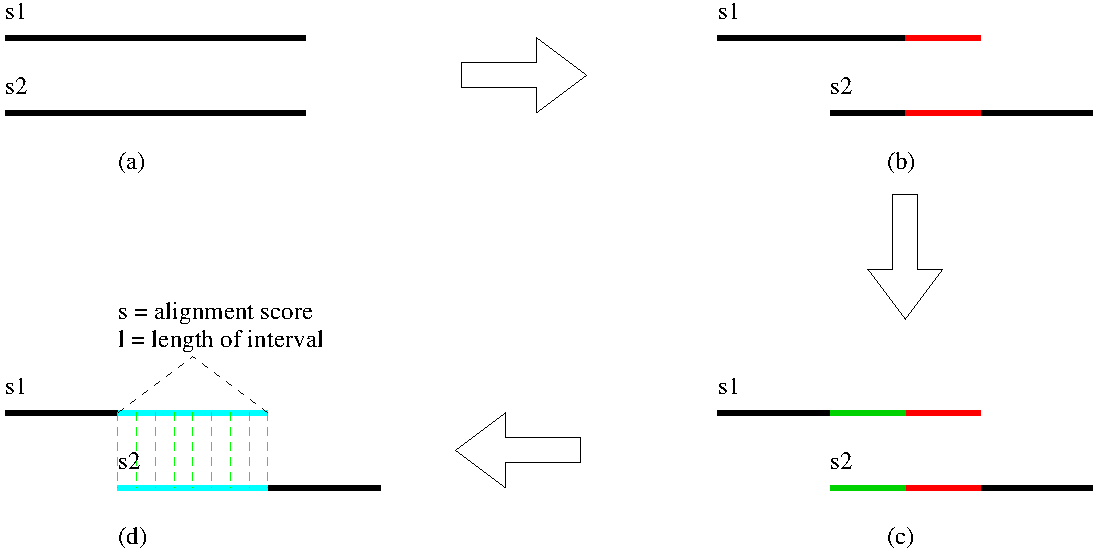
\includegraphics[width=3in]{overlap_alignment.pdf}}
\caption{(a) Two sequences potentially overlapping at the ends.  (b)
  The window of $s_2$ pairing with the right-most window of $s_1$ to
  minimize the $d^2$ score.  (c) An extension of the $s_2$ window to
  the end of the sequence, and the corresponding extension on $s_1$.
  (d) A global alignment of the overlapping areas determined from
  (c).}\label{fig:overlap}
\end{figure}


We note that both \peace\/ and \east\/ make use of an {\it adaptive
  $d^2$} strategy to handle hybrid data sets.  The $d^2$ measure (and
our modification) is flexible enough to handle a range of sequence
sizes, requiring only a modification of the parameters (i.e. window
size and threshold values).  However, it runs into problems when
comparing sequences of significantly different sizes.  Comparing a 62
base Illumina read against a 1000 base Sanger read requires the use of
parameters appropriate to the shorter fragment -- which are
considerably less accurate when applied to the longer read.  Our
solution is to partition fragments by sizes (e.g. into groups of
small, medium and large fragments), and compute distances only
between segments in the name or neighboring groups.  By skipping the
comparisons between sequences of significantly different sizes we
avoid the pitfalls of such comparisons.

\subsection*{Ordering and Reconstruction}

Having defined overlap distance, ordering the fragments is
straight-forward.  We pick an arbitrary node on the cluster's MST and
transverse the tree, using the overlap distance measure to check each
node against its two neighbors.  Those nodes with no identified
left-overlap are checked against nodes further out in the tree, and
any remaining with no identified left-overlap are designated as a contig
left end.

Having identified the distance of each node from its two closest
overlapping sequences, we now construct a {\it directed} graph, with
each edge pointing from a sequence to its right neighbor and weighted
with the overlap distance.  Using this graph we calculate a new
minimum spanning tree, the starting from the root of the tree
(necessarily a left-end of the contig), we transverse the tree and
assign the first base of each sequence a position relative to its
parent.  Such an assignment gives us an implicit ordering of the
fragments, by scanning through them in order and aligning each to
the next with the Smith-Waterman alignment we end up with a multiple
alignment of the fragments that allows us to derive a consensus
sequence.






    
%%%%%%%%%%%%%%%%%%%%%%%%%%%%%%%%
\section*{Authors contributions}
    Text for this section \ldots

    

%%%%%%%%%%%%%%%%%%%%%%%%%%%
\section*{Acknowledgements}
  \ifthenelse{\boolean{publ}}{\small}{}
  Text for this section \ldots


 
%%%%%%%%%%%%%%%%%%%%%%%%%%%%%%%%%%%%%%%%%%%%%%%%%%%%%%%%%%%%%
%%                  The Bibliography                       %%
%%                                                         %%              
%%  Bmc_article.bst  will be used to                       %%
%%  create a .BBL file for submission, which includes      %%
%%  XML structured for BMC.                                %%
%%                                                         %%
%%                                                         %%
%%  Note that the displayed Bibliography will not          %% 
%%  necessarily be rendered by Latex exactly as specified  %%
%%  in the online Instructions for Authors.                %% 
%%                                                         %%
%%%%%%%%%%%%%%%%%%%%%%%%%%%%%%%%%%%%%%%%%%%%%%%%%%%%%%%%%%%%%


{\ifthenelse{\boolean{publ}}{\footnotesize}{\small}
 \bibliographystyle{bmc_article}  % Style BST file
  \bibliography{bmc_article} }     % Bibliography file (usually '*.bib' ) 

%%%%%%%%%%%

\ifthenelse{\boolean{publ}}{\end{multicols}}{}

%%%%%%%%%%%%%%%%%%%%%%%%%%%%%%%%%%%
%%                               %%
%% Figures                       %%
%%                               %%
%% NB: this is for captions and  %%
%% Titles. All graphics must be  %%
%% submitted separately and NOT  %%
%% included in the Tex document  %%
%%                               %%
%%%%%%%%%%%%%%%%%%%%%%%%%%%%%%%%%%%

%%
%% Do not use \listoffigures as most will included as separate files

\section*{Figures}
  \subsection*{Figure 1 - Sample figure title}
      A short description of the figure content
      should go here.

  \subsection*{Figure 2 - Sample figure title}
      Figure legend text.



%%%%%%%%%%%%%%%%%%%%%%%%%%%%%%%%%%%
%%                               %%
%% Tables                        %%
%%                               %%
%%%%%%%%%%%%%%%%%%%%%%%%%%%%%%%%%%%

%% Use of \listoftables is discouraged.
%%
\section*{Tables}
  \subsection*{Table 1 - Sample table title}
    Here is an example of a \emph{small} table in \LaTeX\ using  
    \verb|\tabular{...}|. This is where the description of the table 
    should go. \par \mbox{}
    \par
    \mbox{
      \begin{tabular}{|c|c|c|}
        \hline \multicolumn{3}{|c|}{My Table}\\ \hline
        A1 & B2  & C3 \\ \hline
        A2 & ... & .. \\ \hline
        A3 & ..  & .  \\ \hline
      \end{tabular}
      }
  \subsection*{Table 2 - Sample table title}
    Large tables are attached as separate files but should
    still be described here.



%%%%%%%%%%%%%%%%%%%%%%%%%%%%%%%%%%%
%%                               %%
%% Additional Files              %%
%%                               %%
%%%%%%%%%%%%%%%%%%%%%%%%%%%%%%%%%%%

\section*{Additional Files}
  \subsection*{Additional file 1 --- Sample additional file title}
    Additional file descriptions text (including details of how to
    view the file, if it is in a non-standard format or the file extension).  This might
    refer to a multi-page table or a figure.

  \subsection*{Additional file 2 --- Sample additional file title}
    Additional file descriptions text.


\end{bmcformat}
\end{document}








% LocalWords:  Ozden Chun Liang Karro Botanty publ MSTs et al Hazelhurst Prim's
% LocalWords:  mers Illumina contig bmc multi
